\documentclass{article}
\usepackage{graphicx}
\usepackage{amsmath}

\begin{document}

\title{Backbone Determination in a Wireless Sensor Network}
\author{Jake Carlson}
\date{February 18, 2018}
\maketitle

\abstract
A report on implementing algorithms to partition a random geometric graph into bipartite subgraphs. Three different graph geometries are explored: unit square, unit disk, and unit sphere. Nodes are uniformly distributed in the geometry. Then the edges are determined and ...
\newpage

\tableofcontents
\newpage

\section{Executive Summary}

    \subsection{Introduction}

    \subsection{Environment Description}
    The data structures and topologies for this simulation are implemented in Python2.7. The graphics are done using Processing.py. All development and benchmarking has been done on a 2014 MackBook Pro with a 3 GHz Intel Core i7 processor and 16 GB of DDR3 RAM.

\section{Reduction to Practice}

    \subsection{Data Structure Design}
    The primary data structure used for this project is an adjacency list. However, to allow for constant time lookup of edges of a node, I used a Python dictionary where the keys are nodes and the values are a list of adjacent nodes.

    \subsection{Algorithm Descriptions}

        \subsubsection{Node Placement}
        A different node placement algorithm is required for each of the geometries. For the square, the coordinates for each node are generated as two random numbers taken from a unifrom distribution on the range $0$ - $1$. All of these points are guaranteed to be in the unit square.
        \par
        For the disk, a similar method is used. The coordinates for nodes are randomly sampled from a uniform distribution; however, if a node has a distance from the center of the disk greater than the radius of 1, the coordinates are resampled.
        \par
        For the sphere a different method must be used so that all of the nodes are placed on the surface of the sphere and the volume is vacant. For this geometry, I used the following equations:
        \begin{align}
            x &= \sqrt{1-u^2}\cos\theta \\
            y &= \sqrt{1-u^2}\sin\theta \\
            z &= u
        \end{align}
        where $\theta \in [0,2\pi]$ and $u \in [-1,1]$. This is guaranteed to uniformly distribute nodes on the surface area of the sphere \cite{spherepoints}.

        \subsubsection{Edge Determination}
        I implemented multiple methods for finding the edges in the graph. The brute force method iterates over every node, and for each node checks all other nodes to see if they are close enough to form an edge. The brute force method is $\Theta\left(n^2\right)$ where $n = |V|$.
        \par
        The second method I implemented to find the edges is the sweep method. This method first sorts the nodes along the x-axis. Then, for any node, we only need to search left and right until the distance along the x-axis is greater than the connection radius for the nodes. This dramatically reduces the search space. The sweep method is $O\left(n lg(n) + 2rn^2\right)$ where $n = |V|$ and $r$ is the connection radius. The $n lg(n)$ portion is for the sorting and the $2rn^2$ portion is for measuring the distance between nodes in a sweep step.
        \par
        The final method I implemented to find edges is the cell method. This method places the nodes into cells of area $r \times r$ based on their position in the topology. When the edge detection runs, each node needs to be visited once, but only the cell the node populates and the neighboring cells need to be searched for connections.

        % TODO: update for 3D algos

    \subsection{Algorithm Engineering}

    \subsection{Verification}

    % \subsection{RGG Generation}
    %
    %     \subsubsection{Edge Determination}
    %
    % \subsection{Graph Coloring}
    %
    % \subsection{Backbone Selection}

\section{Results Summary}

\newpage

\begin{thebibliography}{10}
    \bibitem{spherepoints}
    Weisstein, Eric W., Wolfram MathWorld
    \textit{Sphere Point Picking}
    \texttt{http://mathworld.wolfram.com/SpherePointPicking.html}

\end{thebibliography}

\newpage

\section{Appendix}

\begin{center}
    \begin{figure}
        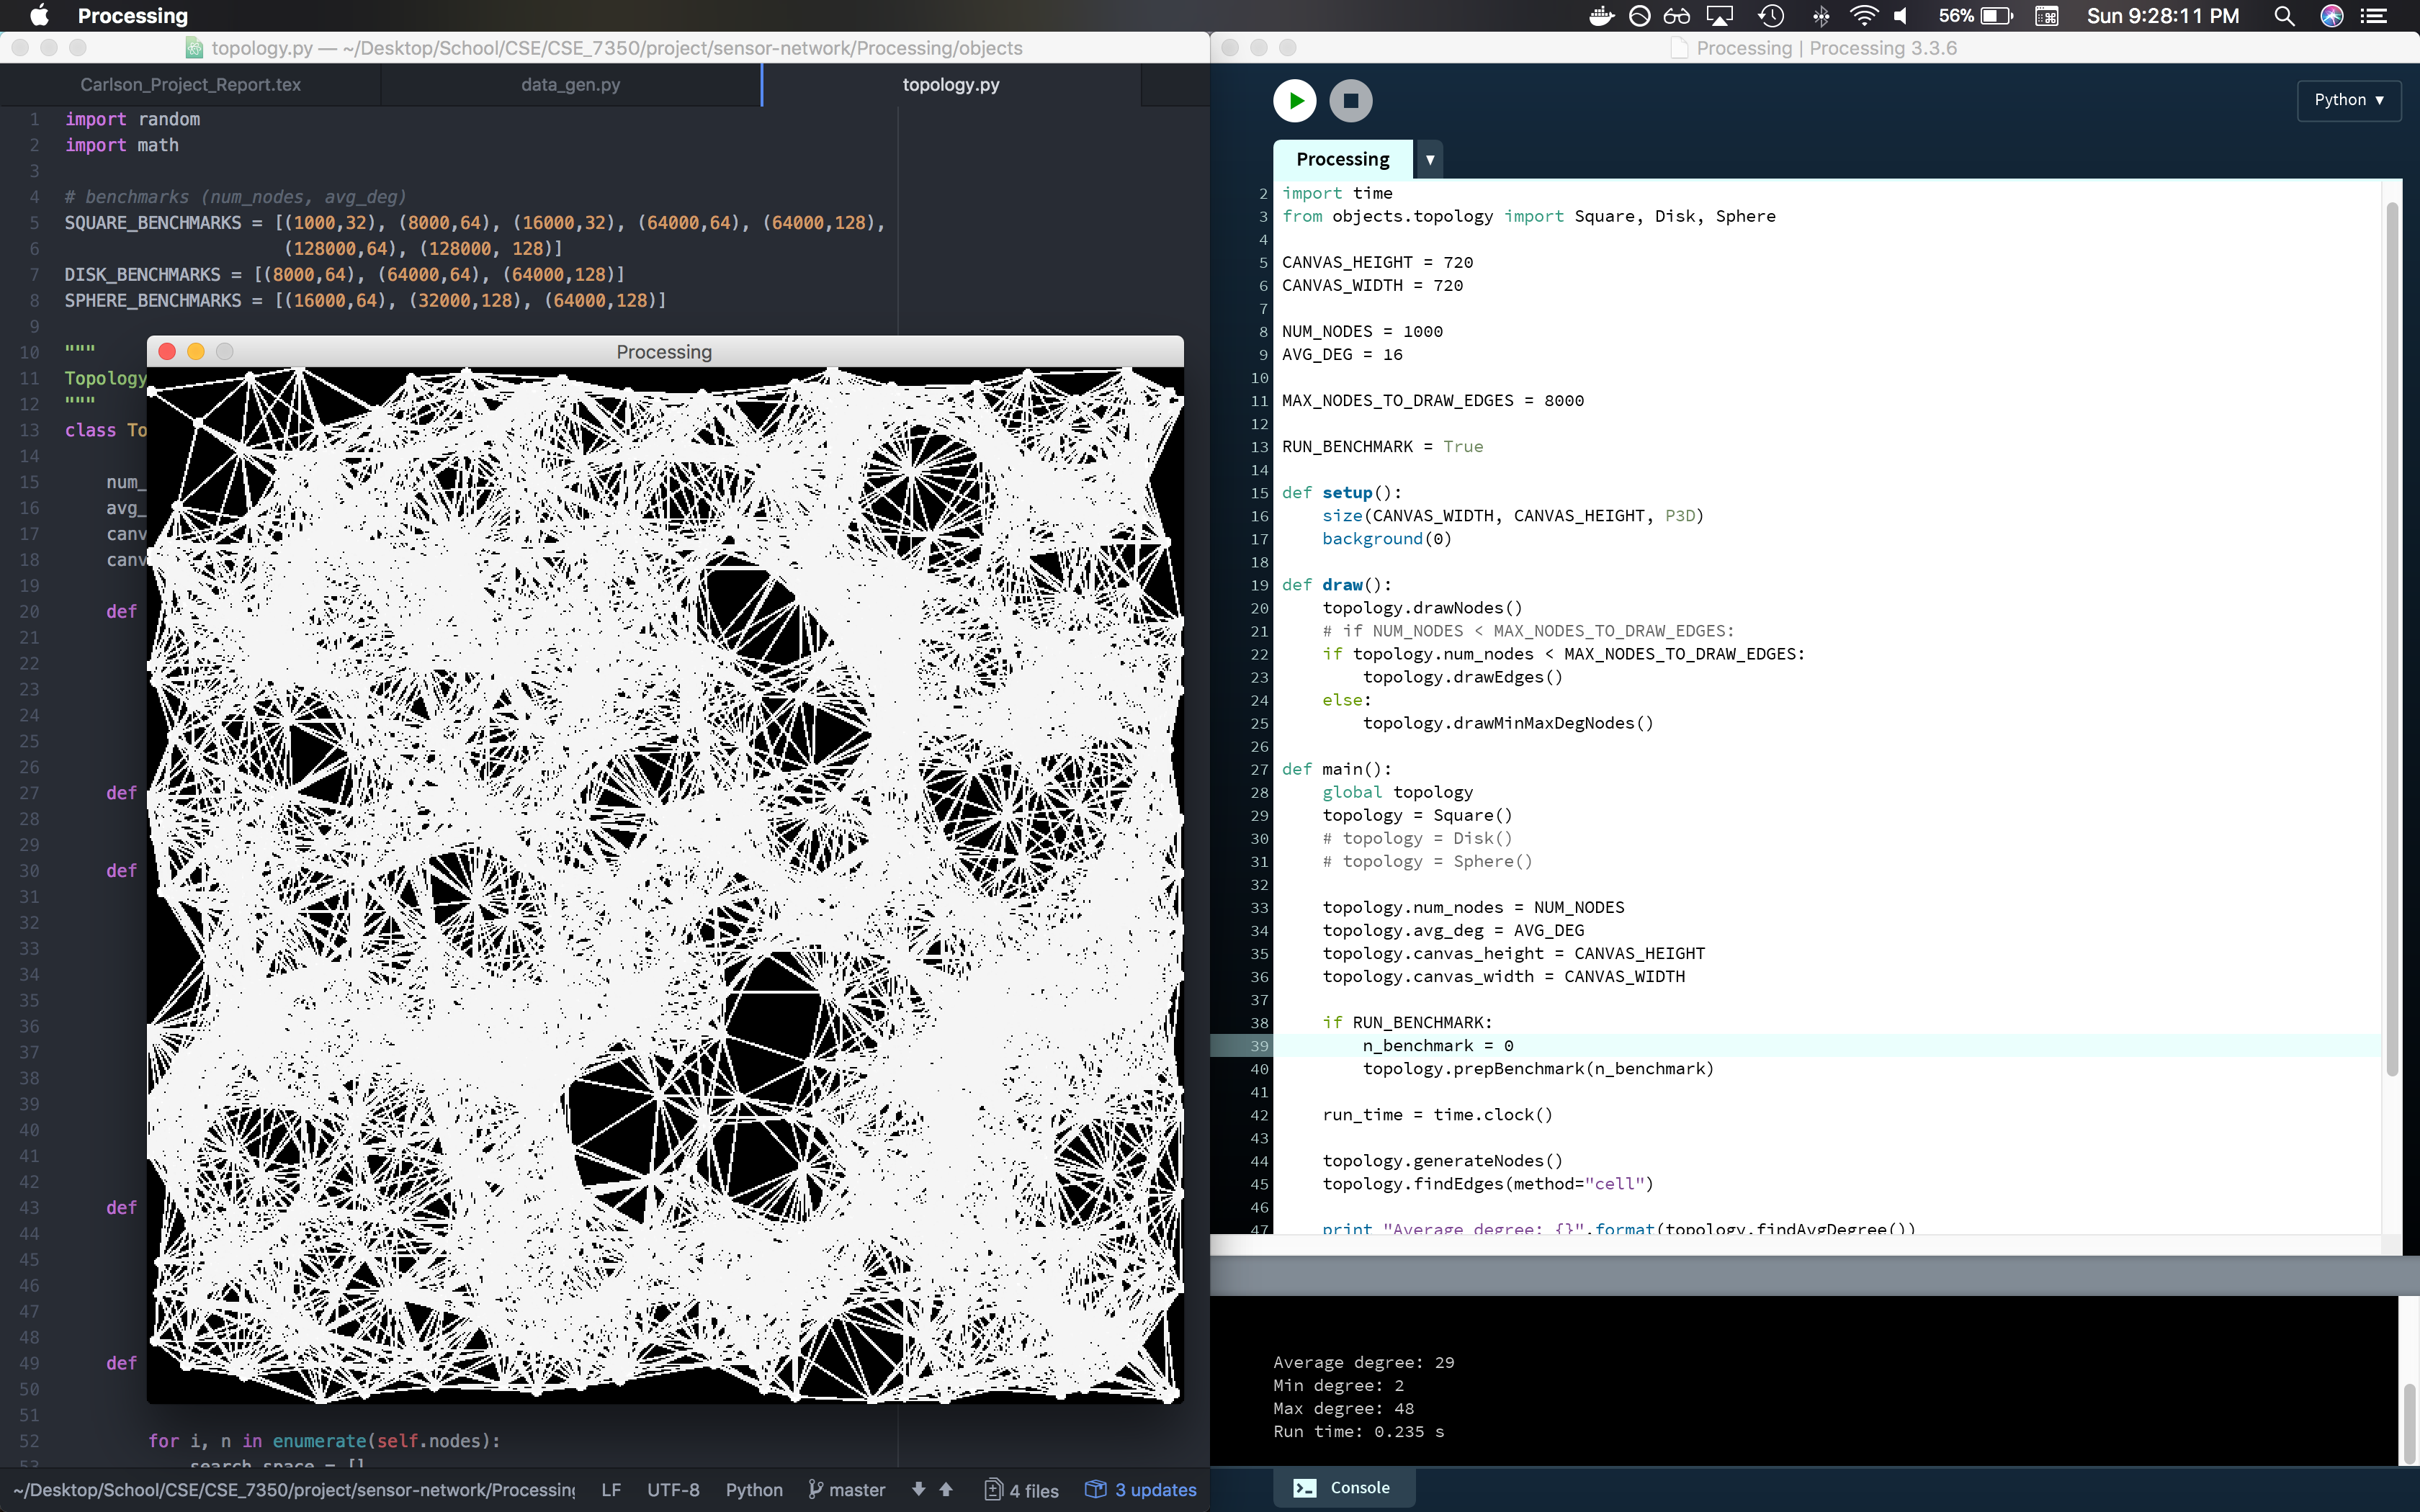
\includegraphics[scale=0.25]{./images/square_0.png}
        \caption{Square Benchmark Number 0. 1000 Nodes, Average Degree of 32}
        \label{square0}
    \end{figure}
\end{center}

\end{document}
